In a study conducted by Harris Interactive \cite{Harris} among 2.311 U.S. adults ages 18 and over, on how they use and feel about interaction on the internet. It was conducted between April 28 and 30 2010. They asked different question and some of them are quite interesting.
Although it was conducted in America, the information can still be used in our project. The idea behind our project is to create a website that can be accessed from across the world. So different studies in different countries are useful for the information needed to determine the target group. That is why this information is useful for our project.

The first graph asks the question about what the asked person shares through social media. They were to select all that applies to them. If we take a look on what the different options was, one stands out and that is: TV and movie recommendations. In the range from 18 to 34 year old, 36 percent of them says that they share TV and movie recommendations on social media.

\begin{figure}[htb]
\centering
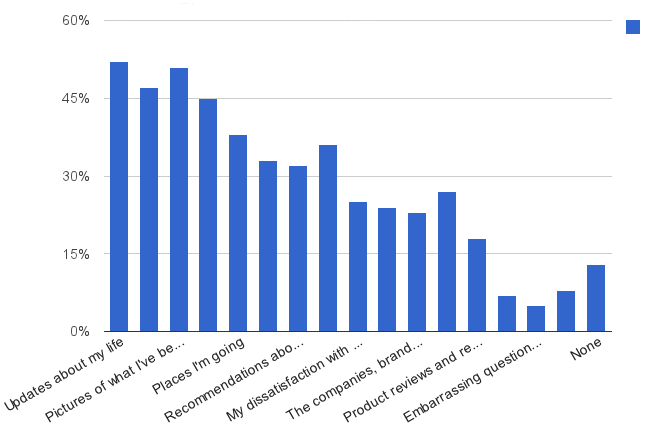
\includegraphics[width=0.8\textwidth]{Images/teori1.png}
\caption{1}
\label{Teori1}
\end{figure}

The first interesting question and answer is, that in short terms asks what the person share on social media and select all that applies. If we take a look on what the different options were one strikes out and that is; TV and movie recommendations. In the range from 18 to 34 year olds, 36 percent of them says that they share TV and movie recommendations on social media.

The second graph pose the question about how much different reviews from different people influence them. It shows that 71 percent of those asked replied that they are influenced a great deal or a fair amount by reviews from family members or friends. 

\begin{figure}[htb]
\centering
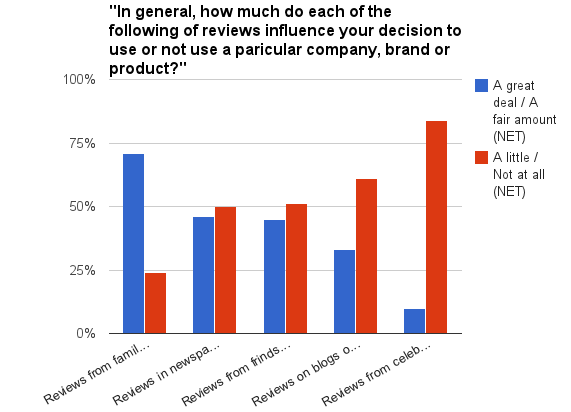
\includegraphics[width=0.8\textwidth]{Images/teori2.png}
\caption{1}
\label{Teori2}
\end{figure}

The second graph asks the question about how much different things influence them. It shows that a staggering 71 percent of those asked, replied that they are influenced a great deal or a fair amount by reviews from family members or friends. That shows that social recommendation is something that a lot of people have in mind when it comes to buy or watch something.

The third and last graph shows the age group of those asked the previous question. That graph shows that the 18 to 34 year olds are more influenced by blog and social media, than the older ages were. At the same time, the older people are more influenced by their family and friends.

\begin{figure}[htb]
\centering
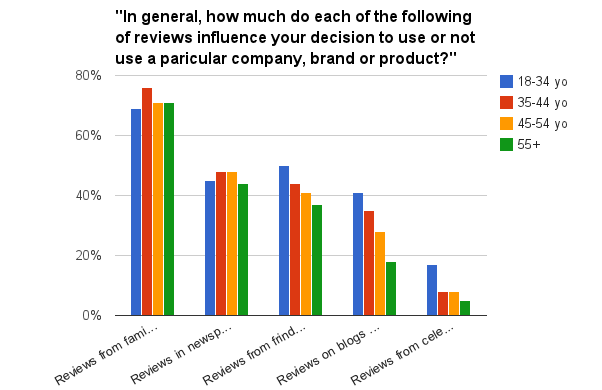
\includegraphics[width=0.8\textwidth]{Images/teori3.png}
\caption{1}
\label{Teori3}
\end{figure}

The third and last graph shows the age group of those asked the previous question. It shows that 18-34 year old are more influenced by blogs and social media than the older ages. While the older people have are more influenced by their family and friends.